\documentclass[11pt]{exam}
\usepackage[activeacute,spanish]{babel} % Permite el idioma espa\~nol.
\usepackage[utf8]{inputenc}
\usepackage{amsmath,amsfonts}
\usepackage[colorlinks]{hyperref}
\usepackage{graphicx}

\pagestyle{headandfoot}

\spanishdecimal{.}
%se redefine comando que cita figuras
\newcommand{\figref}[1]{\ref{#1}}
\usepackage{float}%para poder poner figuras justo en el lugar que deseo con \begin{figure}[H]
\begin{document}

\firstpageheadrule
%\firstpagefootrule
%\firstpagefooter{}{Pagina \thepage\ de \pages}{}
\runningheadrule
%\runningfootrule
\lhead{\bf\normalsize Taller Python 2019}
\rhead{\bf\normalsize Tarea \'area Ingenier\'ia}
\cfoot{ }
\lfoot{\tiny NNIV}
\begin{flushleft}
\vspace{0.2in}
%\hbox to \textwidth{Nombre: \enspace \hrulefill}
%Nombre : \\
\vspace{0.25cm}
\end{flushleft}
%%%%%%%%%%%%%%%%%%%%%%%%%%%%%%%%%%%%%%%%%%

\begin{center}
\textbf{Fecha M'axima de entrega: Lunes 21 de Enero}
\end{center}
\textbf{Instrucciones:} Resuelva el problema propuesto usando Python. Env'ie todos los archivos necesarios para reproducir sus resultados (archivos de datos, c'odigos .py, notebooks .ipynb, etc.) por email a \texttt{nibarra@ubiobio.cl}.

\bigskip
El algoritmo tradicional que transforma una imagen a la escala de grises es la que promedia los valores cada canal de color (rojo, verde y azul) mediante la relaci\'on \eqref{eq:x_promedio} y asigna a cada canal dicho promedio $x$.
\def \rojo{\color{red}{\text{rojo}}}
\def \verde{\color{green}{\text{verde}}}
\def \azul{\color{blue}{\text{azul}}}
\def \plus{\color{black}{+}}
\def \coma{\color{black}{,}}
\begin{align}
x = \color{green}{\text{int}} \color{black} 
\left(\frac{ \rojo \plus \verde \plus \azul}{3}\right). \label{eq:x_promedio}
\end{align}

En otras palabras, si un pixel de la imagen tiene asociados los valores
\begin{align}
\text{pixel} = (\rojo \coma\, \verde \coma\, \azul), 
\end{align}
el nuevo pixel tendr\'a los valores:
\begin{align}
\text{nuevo pixel} = (x,\, x,\, x).
\end{align}

Una mejor elecci\'on para la escala de grises es la \href{https://es.wikipedia.org/wiki/UIT-R_BT.601-7}{\textbf{ITU-R Recommendation BT.601-7}}, la cual especifica m\'etodos para codificar digitalmente se\~nales de video mediante normalizaci\'on de valores. Para la transmisi\'on de escala de grises define la f\'ormula de la ec. \eqref{eq:x_ITU}.
\begin{align}
x = \color{green}{\text{int}} \color{black}(0.299 \times \rojo \plus 0.587 \times \verde \plus 0.114 \times \azul \color{black}). \label{eq:x_ITU}
\end{align}

\begin{itemize}
\item Desde \href{https://github.com/PythonUdeC/CPC19/blob/master/images/IMG_20190109_144618.jpg}{aqu\'i} descargue la fotograf\'ia del curso y c\'arguela con la funci\'on \texttt{imageio.imread}.
\item Escriba una funci\'on que tenga como \texttt{input} la imagen y como \texttt{output} la imagen convertida a la escala de grises usando la ec. \eqref{eq:x_promedio}.
\item Escriba una funci\'on que tenga como \texttt{input} la imagen y como \texttt{output} la imagen convertida a la escala de grises usando la ec. \eqref{eq:x_ITU}.
\item Con la funci\'on \texttt{matplotlib.pyplot.imshow} visualice las im\'agenes en ambas escalas de grises. Note que deben lucir como se muestra en la figura \figref{fig:escalas_grises}. En su correo responda \textquestiondown cu\'al algoritmo le gust\'o m\'as?
\item Con la funci\'on \texttt{imageio.imsave} guarde las nuevas im\'agenes.
\item Finalmente, t\'omese una selfie y repita el proceso. Puede subir las im\'agenes convertidas a sus redes sociales jact\'andose de haber codificado los filtros con sus propias manitos en \texttt{Python}.
\end{itemize}
\begin{figure}[H]
 \centering
% \includegraphics[width=7.5cm]{../images/IMG_20190109_144618.jpg}
 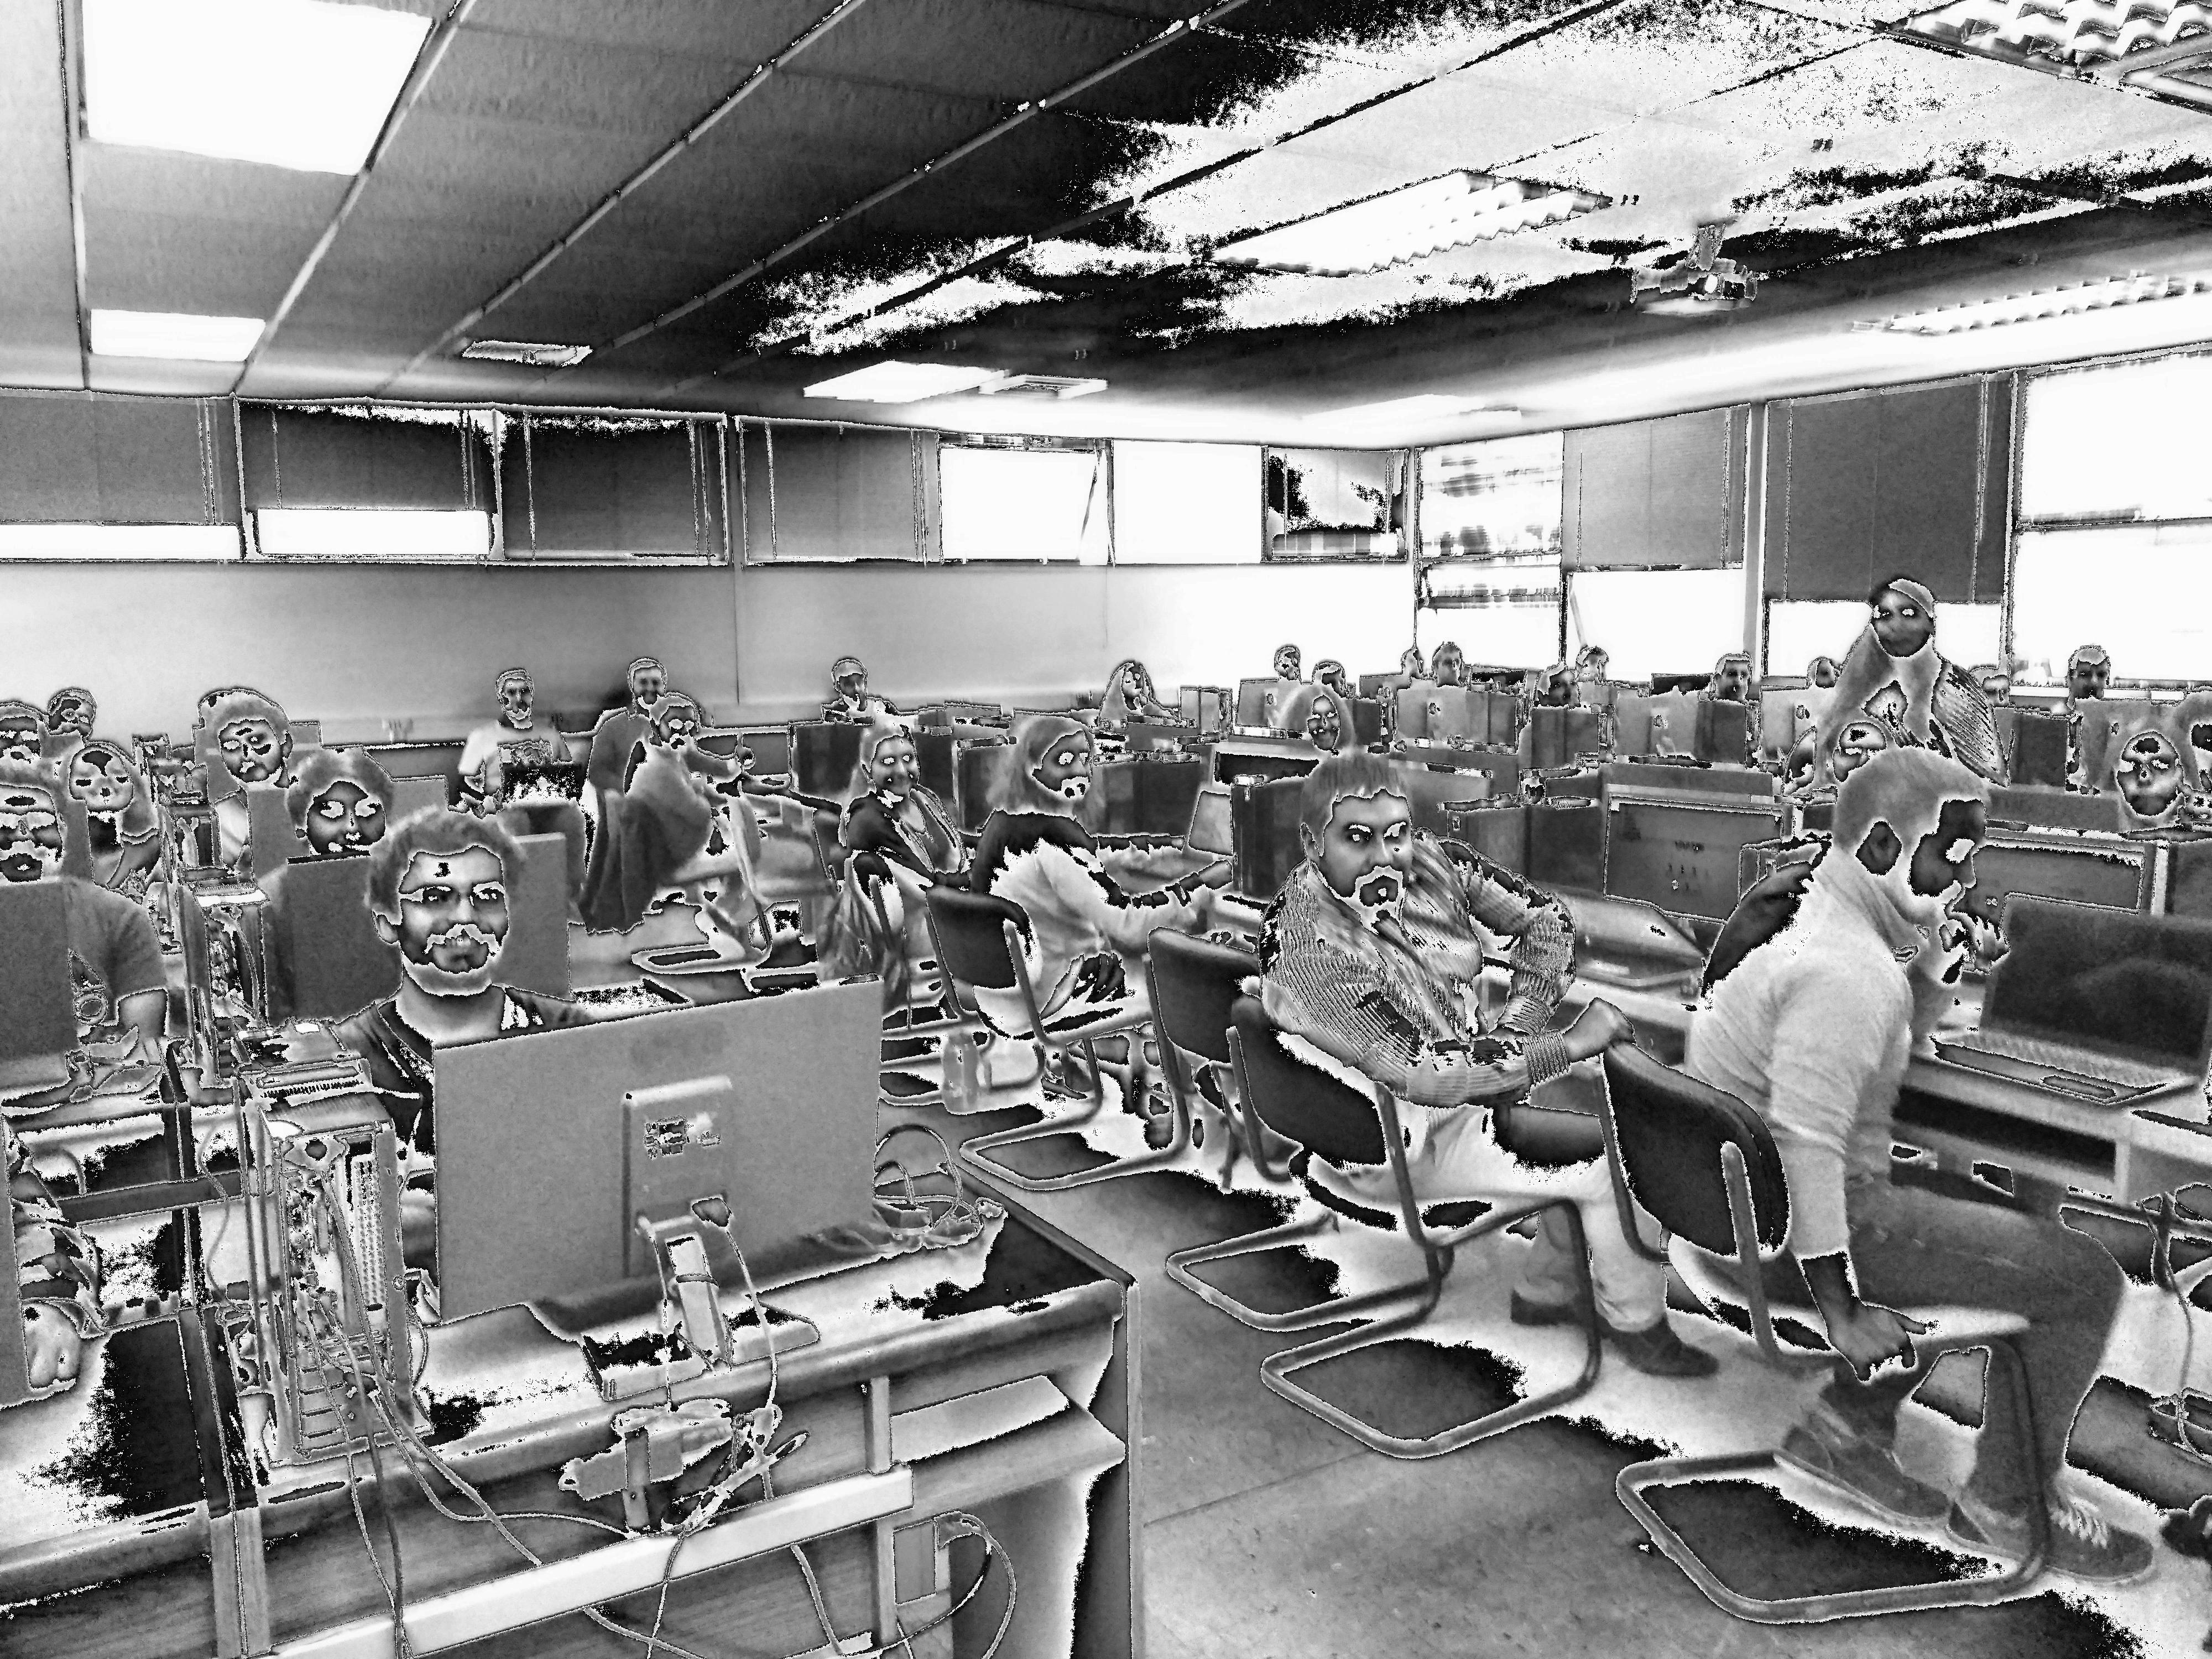
\includegraphics[width=7.5cm]{../images/curso_gris01.jpg}
 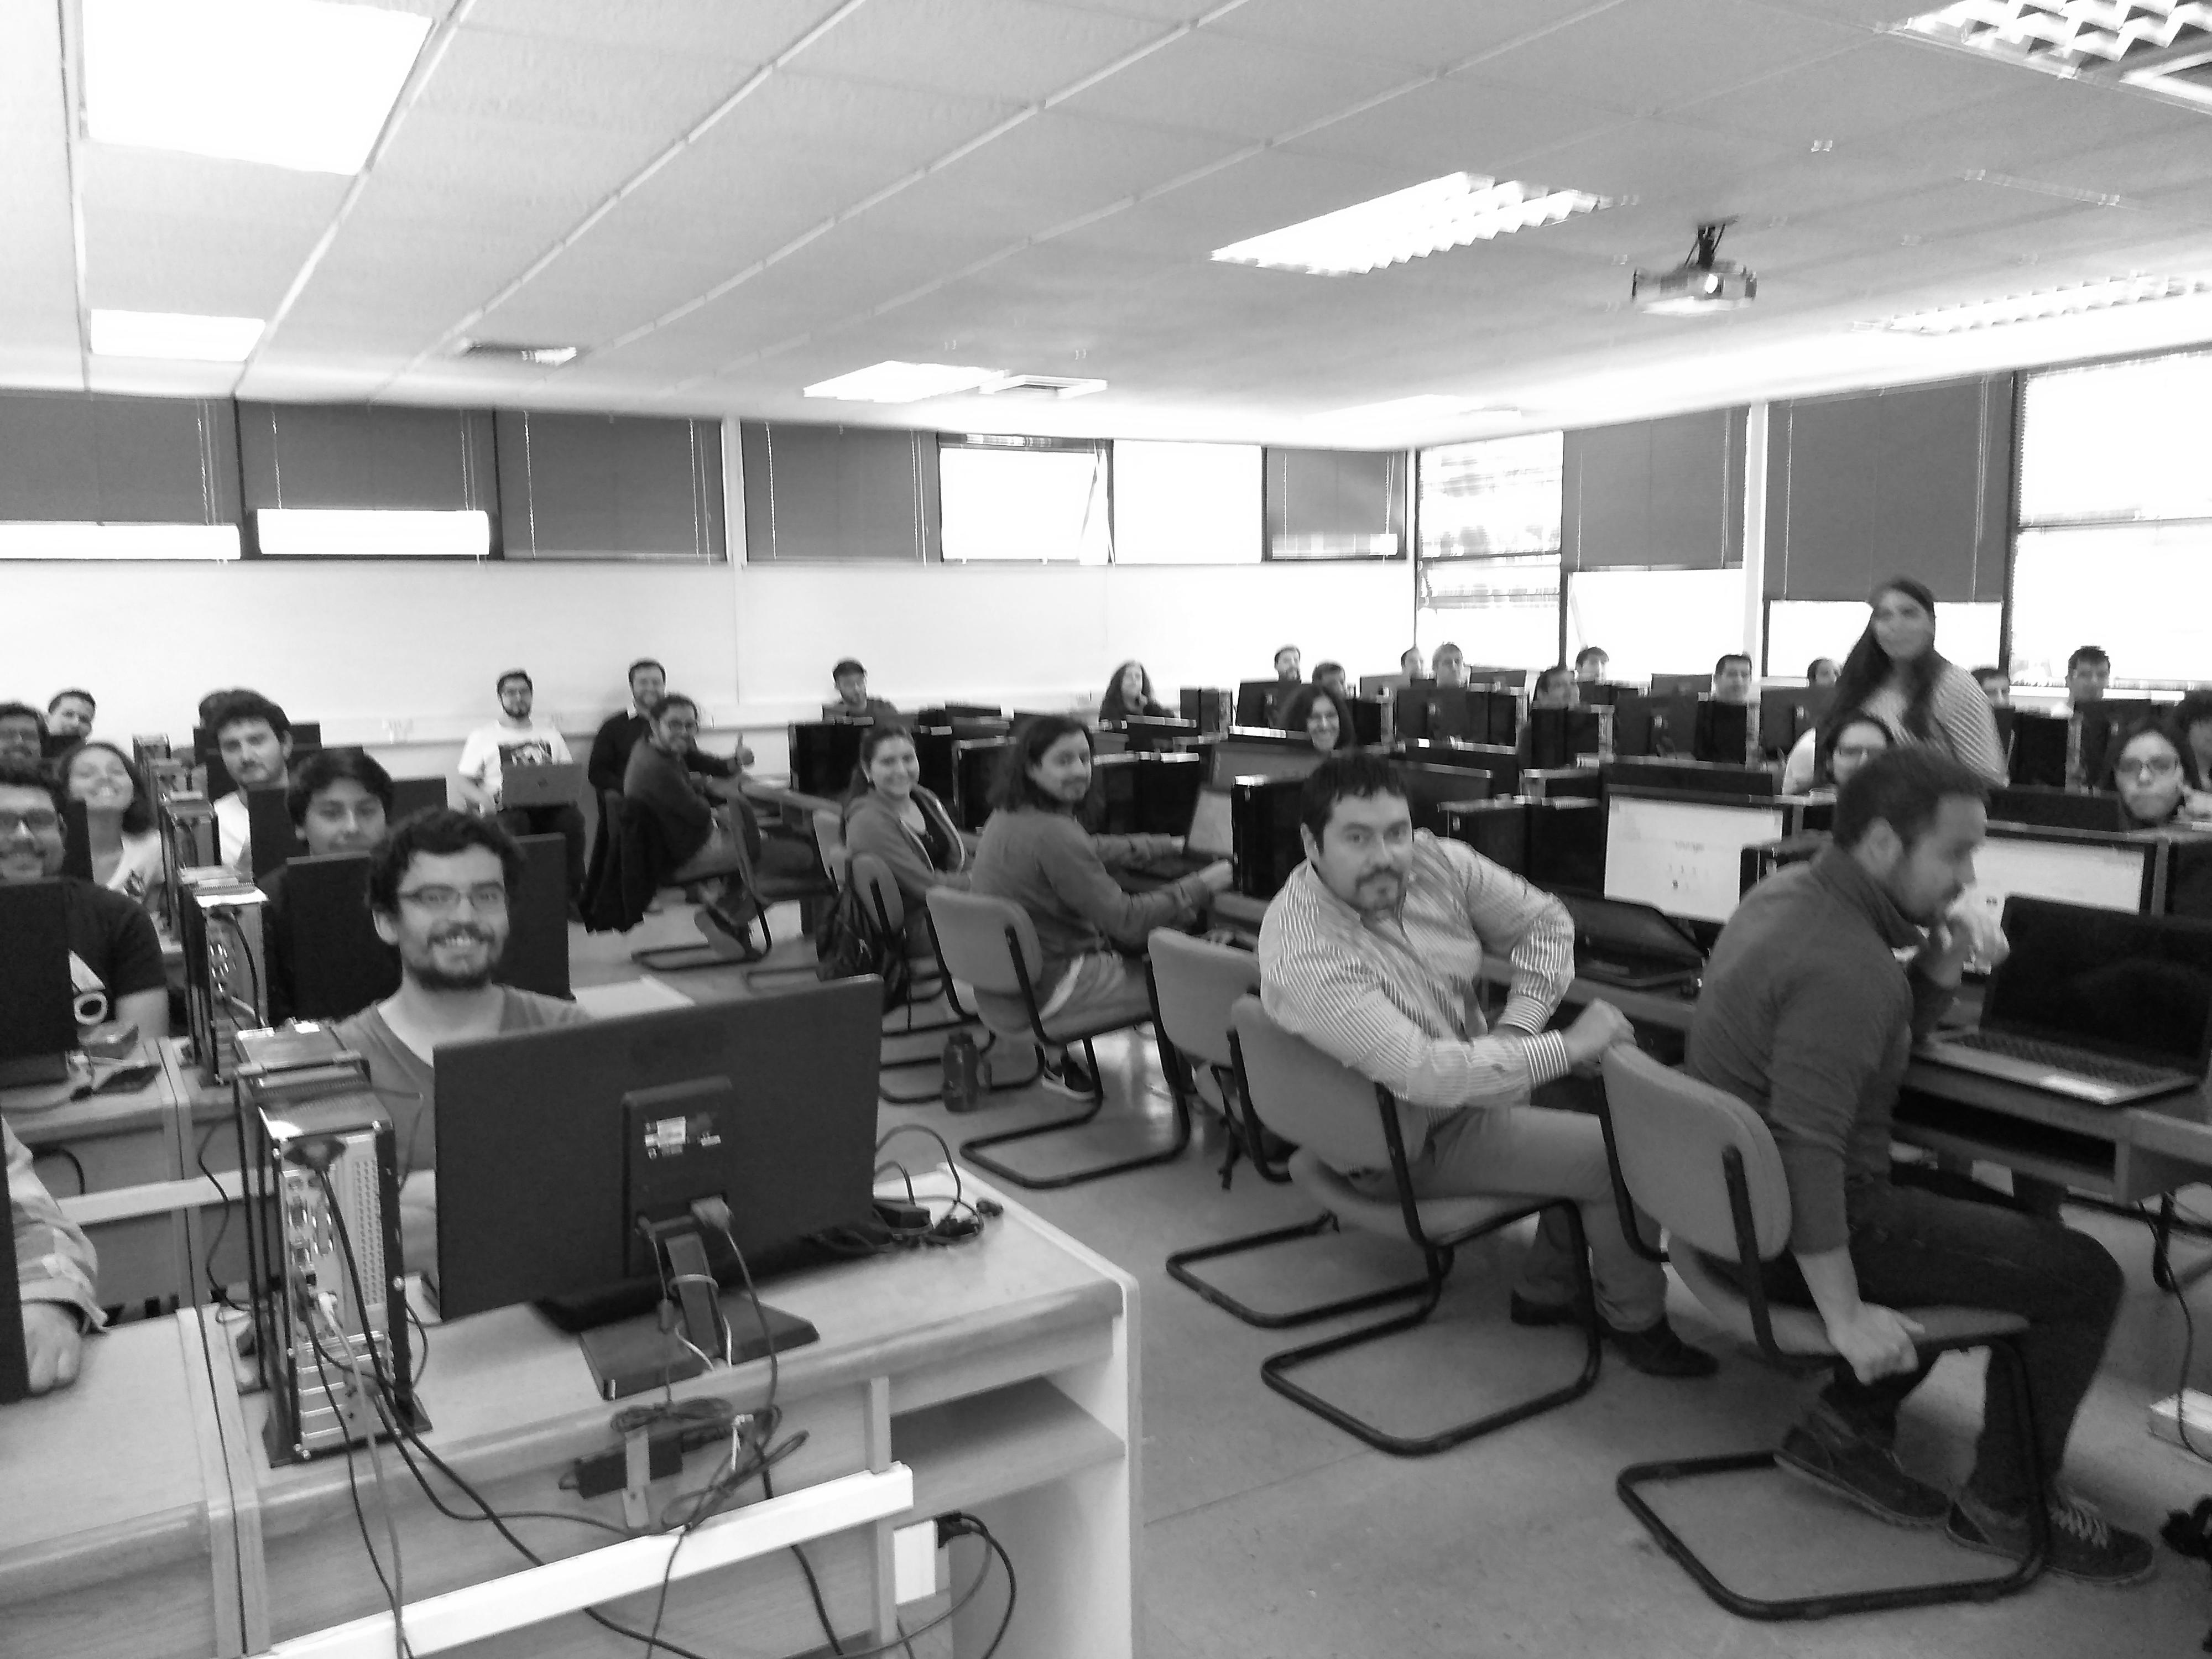
\includegraphics[width=7.5cm]{../images/curso_gris02.jpg}
 \caption{Conversi\'on de imagen a distintas escalas de grises.}
 \label{fig:escalas_grises}
\end{figure} 

\end{document} 
